\begin{figure}[H]
\centering
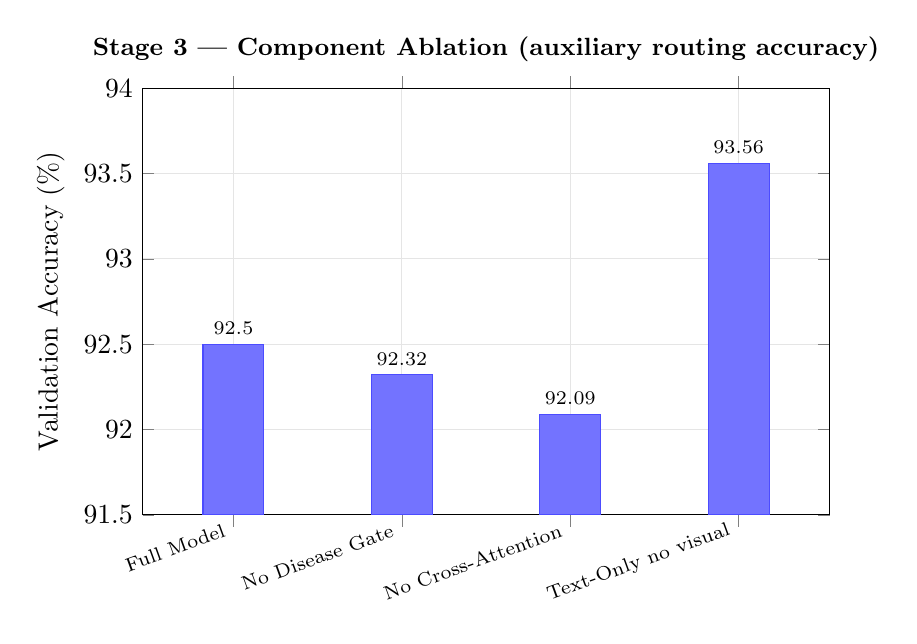
\begin{tikzpicture}
\begin{axis}[ybar, width=0.85\linewidth, height=7cm,
    title={\textbf{Stage 3 --- Component Ablation (auxiliary routing accuracy)}},
    title style={font=\small\bfseries},
    ylabel={Validation Accuracy (\%)}, ymin=91.5, ymax=94,
    symbolic x coords={Full Model,No Disease Gate,No Cross-Attention,Text-Only no visual}, xtick=data,
    x tick label style={rotate=20, anchor=east, font=\scriptsize},
    nodes near coords, nodes near coords style={font=\scriptsize,
        /pgf/number format/fixed, /pgf/number format/precision=2},
    bar width=22pt, grid=major, grid style={gray!20},
    enlarge x limits=0.18]
\addplot[fill=blue!55, draw=blue!70] coordinates {(Full Model,92.50) (No Disease Gate,92.32) (No Cross-Attention,92.09) (Text-Only no visual,93.56)};
\end{axis}\end{tikzpicture}
\caption[Stage 3 ablation]{Stage~3 component ablation on the auxiliary routing
head. Removing the disease gate or cross-attention costs only 0.18 and 0.41
percentage points respectively. Notably, a text-only variant marginally
\emph{exceeds} the full model on this routing metric (93.56\% vs 92.50\%),
confirming that question-type routing is essentially a textual task; the visual
and disease signals are introduced for the benefit of downstream answer
generation (Stage~4), not for routing.}
\label{fig:stage3_ablation}
\end{figure}
